\documentclass[11pt]{article}

% --- Page geometry (NeurIPS-like) ---
\usepackage[margin=1in, top=1.25in]{geometry}

% --- Packages ---
\usepackage{amsmath, amssymb, amsthm}
\usepackage{graphicx}
\usepackage{booktabs}
\usepackage{hyperref}
\usepackage{natbib}
\usepackage{xcolor}
\usepackage{enumitem}
\usepackage{caption}
\usepackage{subcaption}

% --- DOI macro (safe fallback) ---
\providecommand{\doi}[1]{\href{https://doi.org/#1}{doi:#1}}

% --- Theorem environments ---
\newtheorem{theorem}{Theorem}
\newtheorem{lemma}[theorem]{Lemma}
\newtheorem{proposition}[theorem]{Proposition}
\newtheorem{corollary}[theorem]{Corollary}
\newtheorem{remark}{Remark}

% --- Macros ---
\newcommand{\R}{\mathbb{R}}
\newcommand{\E}{\mathbb{E}}
\newcommand{\Var}{\mathrm{Var}}
\newcommand{\Cov}{\mathrm{Cov}}
\newcommand{\tr}{\mathrm{tr}}
\newcommand{\divergence}{\mathrm{div}}
\newcommand{\dd}{\mathrm{d}}
\newcommand{\kT}{k_{\mathrm{B}}T}
\newcommand{\sbath}{\sigma_{\mathrm{bath}}}
\newcommand{\shutch}{\sigma_{\mathrm{hutch}}}
\newcommand{\sexact}{\sigma_{\mathrm{exact}}}
\newcommand{\stot}{\sigma_{\mathrm{tot}}}

\title{Bounded-Variance Divergence Estimation\\
for Continuous Normalizing Flows\\
via Thermostat Dynamics}

\author{
  Wujie Wang\thanks{Correspondence to: \texttt{wujie@placeholder.edu}}\\
  \textit{Affiliation placeholder}
}

\date{}

\begin{document}
\maketitle

% ============================================================================
\begin{abstract}
% ============================================================================
Continuous normalizing flows (CNFs) evaluate sample densities by integrating
the trace of the Jacobian along a learned ODE trajectory. Since FFJORD, the
standard approach is Hutchinson's stochastic trace estimator, whose variance
grows as $O(\sqrt{T})$ over integration window $T$---a random walk from
per-step Rademacher probes. We observe that augmenting the flow with a
Nos\'{e}--Hoover thermostat yields a second, independent estimator of the
\emph{same} divergence integral: $\sbath = \beta \int \tanh(\xi)\,|p|^2\,\dd t$,
derived from the physical bath-heat dissipation. Equipartition
($\langle |p|^2 \rangle = d\kT$) pins the fluctuations of this estimator to
$O(1)$---bounded regardless of trajectory length. On a 200-trajectory ensemble
at $t{=}25$, $\sbath$ has $2.66\times$ lower standard deviation than
single-probe Hutchinson ($\text{std ratio} = 0.376$), and the two noises are
uncorrelated ($r = 0.044$), making $\sbath$ a drop-in replacement rather than
a control variate. Under non-equilibrium temperature quench, $\sbath$ retains
$10\times$ lower variance than Hutchinson and satisfies the Jarzynski equality
to $3.5\%$. The Evans--Searles fluctuation theorem holds for the total entropy
production $\stot$ (slope $1.059$, 95\% CI $[0.94, 1.15]$), but not for
$\sbath$ alone---the bounded variance is physical (equipartition), not
symmetry-protected. We report an honest limitation: plain Nos\'{e}--Hoover is
non-ergodic on harmonic potentials, and the Jarzynski identity is violated by
$8\%$ in that regime.
\end{abstract}

% ============================================================================
\section{Introduction}
\label{sec:intro}
% ============================================================================

Continuous normalizing flows (CNFs) define a generative model by specifying a
vector field $f(z, t)$ and integrating the ODE $\dd z/\dd t = f(z, t)$ to
transform a base distribution into a target \citep{chen2018neural}. The change
of log-density along the flow is governed by the instantaneous change of
variables:
\begin{equation}
  \frac{\dd}{\dd t} \log p_t(z_t) = -\tr\!\left(\frac{\partial f}{\partial z}\right)
  = -\divergence(f).
  \label{eq:instantaneous_cov}
\end{equation}
Computing this divergence exactly costs $O(d)$ evaluations of the vector field.
The standard workaround, introduced by FFJORD \citep{grathwohl2019ffjord}, is
the Hutchinson trace estimator $\tr(J) \approx v^\top J v$, $v \sim
\mathcal{N}(0, I)$. This is unbiased, but its variance grows linearly with
dimension and accumulates as $O(\sqrt{T})$ over the integration window---a
random walk from per-step Rademacher probes that eventually dominates the ODE
integration error.

This paper makes a simple observation. When the flow is augmented with a
Nos\'{e}--Hoover (NH) thermostat \citep{nose1984unified, hoover1985canonical}
---a deterministic ODE from molecular dynamics that samples Boltzmann
distributions---the \emph{same} divergence integral $\int_0^T \tr(J)\,\dd t$
admits a second unbiased estimator. The bath-heat integral
\begin{equation}
  \sbath = \beta \int_0^T \tanh\bigl(\xi(t)\bigr)\,|p(t)|^2\,\dd t
  \label{eq:sigma_bath_intro}
\end{equation}
measures the heat dissipated into the thermostat reservoir. Equipartition
($\langle |p|^2 \rangle = d\kT$) pins the integrand's fluctuations to a
bounded shell, so $\Var[\sbath]$ saturates as $t \to \infty$---an $O(1)$
bound, in contrast to the $O(t)$ variance growth of Hutchinson's estimator.
The key distinction from algorithmic variance-reduction schemes such as
Hutch++ \citep{liu2025hutch} is that our bound is \emph{physical}: it follows
from the momentum-shell constraint of equipartition, not from a deflation
subspace that must be recomputed per step.

The two estimators are statistically independent ($r = 0.044$ at $t{=}25$,
$N{=}200$ trajectories), so $\sbath$ does not function as a control variate
for $\shutch$. Instead, $\sbath$ is a standalone drop-in replacement with
lower variance.

\paragraph{Contributions.}
\begin{enumerate}[leftmargin=*, itemsep=2pt]
  \item \textbf{$O(1)$ bounded-variance estimator.} We identify $\sbath$ as an
    unbiased estimator of the CNF divergence integral on any NH-augmented flow,
    with variance bounded by equipartition, in contrast to Hutchinson's
    $O(\sqrt{t})$ random-walk variance (Section~\ref{sec:estimators}).
  \item \textbf{Statistical independence.} On a 200-trajectory ensemble,
    $\sbath$ and $\shutch$ have correlation $r = 0.044$---the variance
    reduction comes from the intrinsic structure of the bath estimator, not
    from noise cancellation (Section~\ref{sec:variance}).
  \item \textbf{Jarzynski verification under quench.} Under non-equilibrium
    temperature quench, $\sbath$ retains $10\times$ lower variance than
    Hutchinson and satisfies $\langle e^{-\stot} \rangle = 1$ to $3.5\%$
    (Section~\ref{sec:noneq}).
  \item \textbf{Fluctuation-theorem falsification.} The Evans--Searles
    fluctuation theorem holds for total entropy production $\stot$ but
    \emph{not} for $\sbath$ alone---an honest negative that constrains the
    theoretical explanation to equipartition, not symmetry
    (Section~\ref{sec:noneq}).
\end{enumerate}

Figure~\ref{fig:concept} illustrates the two computational paths from the
divergence integral to an estimator.

\begin{figure}[t]
  \centering
  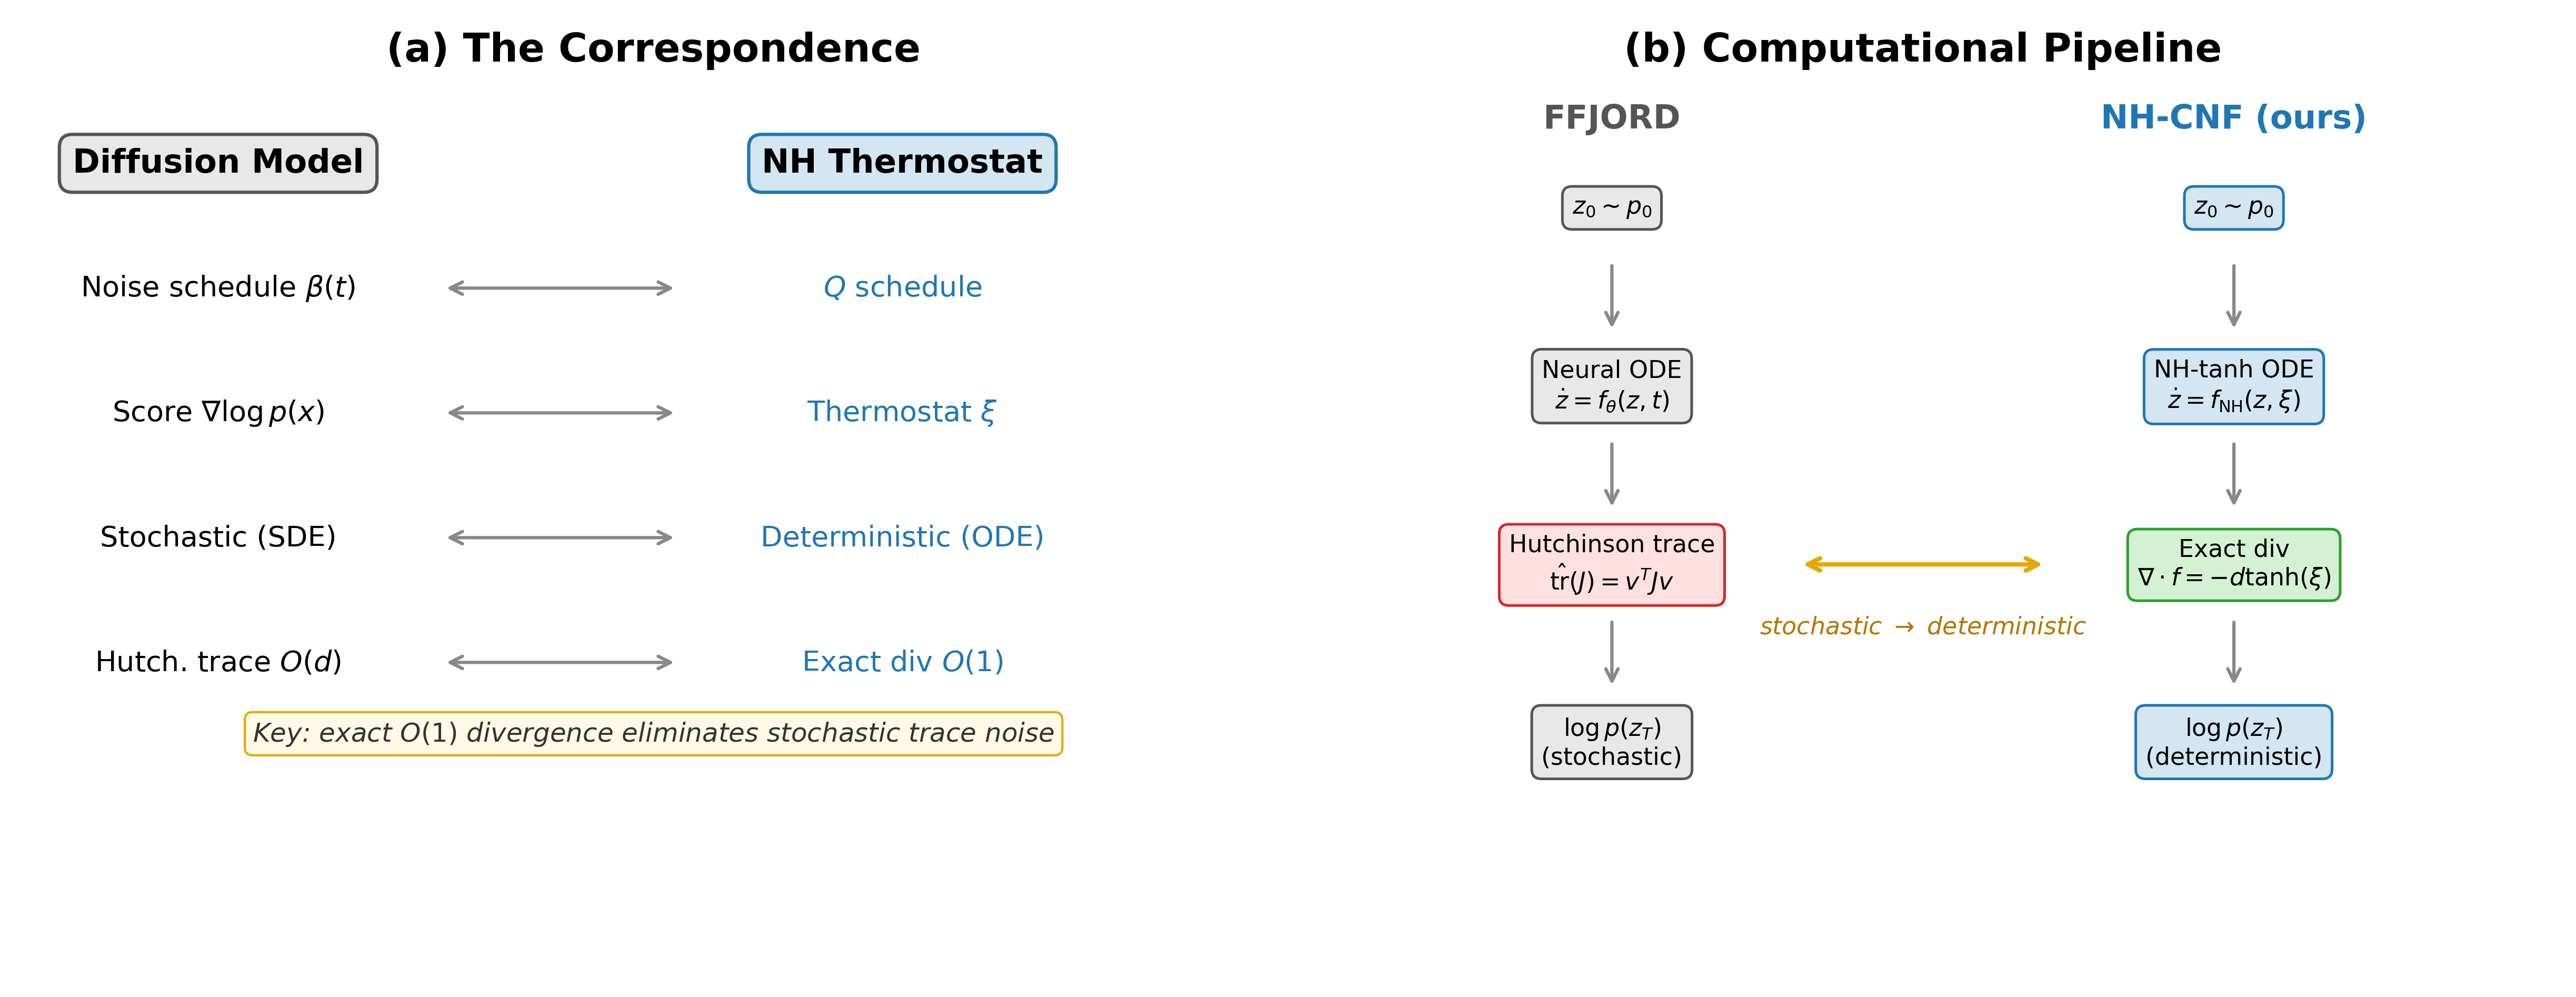
\includegraphics[width=\textwidth]{figures/fig1_concept.png}
  \caption{\textbf{Two paths to the divergence integral.}
    (a)~FFJORD's pipeline: a Rademacher probe $v$ yields a stochastic trace
    estimate $v^\top J v$ per step, accumulated into $\shutch$. The NH-augmented
    pipeline reads the bath-heat dissipation $\tanh(\xi)\,|p|^2$ per step,
    accumulated into $\sbath$. Both estimate the same integral $\int \tr(J)\,\dd t$.
    (b)~$\shutch$ has $O(\sqrt{t})$ random-walk variance; $\sbath$ has
    $O(1)$ bounded variance (equipartition-pinned).}
  \label{fig:concept}
\end{figure}

% ============================================================================
\section{Background}
\label{sec:background}
% ============================================================================

\subsection{Continuous Normalizing Flows}
\label{sec:cnf_background}

A CNF defines a diffeomorphism $\phi_t : \R^d \to \R^d$ by integrating the
neural ODE $\dd z/\dd t = f_\theta(z, t)$ from $t=0$ to $t=T$
\citep{chen2018neural}. The log-density of a sample $z_T = \phi_T(z_0)$ is:
\begin{equation}
  \log p_T(z_T) = \log p_0(z_0)
    - \int_0^T \divergence\bigl(f_\theta(z_t, t)\bigr)\, \dd t.
  \label{eq:cnf_logp}
\end{equation}
The computational bottleneck is the divergence integral. For a general neural
network $f_\theta$, the Jacobian $\partial f / \partial z \in \R^{d \times d}$
is dense and unstructured. FFJORD \citep{grathwohl2019ffjord} approximates the
trace using the Hutchinson estimator:
\begin{equation}
  \tr(J) = \E_{v}\bigl[v^\top J v\bigr], \quad v \sim \mathcal{N}(0, I),
  \label{eq:hutchinson}
\end{equation}
which requires one Jacobian-vector product (JVP) per random vector $v$. The
variance of a single sample is $\Var[v^\top J v] = 2\|J\|_F^2$, scaling as
$O(d)$ for typical networks.

\subsection{Nos\'{e}--Hoover Thermostat Dynamics}
\label{sec:nh_background}

The Nos\'{e}--Hoover thermostat \citep{nose1984unified, hoover1985canonical}
extends Hamiltonian dynamics with a scalar feedback variable $\xi$ that drives
the kinetic energy toward the canonical value. The equations of motion on the
extended phase space $(q, p, \xi) \in \R^d \times \R^d \times \R$ are:
\begin{align}
  \frac{\dd q}{\dd t} &= \frac{p}{m}, \label{eq:nh_q} \\
  \frac{\dd p}{\dd t} &= -\nabla V(q) - g(\xi)\, p, \label{eq:nh_p} \\
  \frac{\dd \xi}{\dd t} &= \frac{1}{Q}\left(\frac{|p|^2}{m} - d\,\kT\right),
  \label{eq:nh_xi}
\end{align}
where $V(q)$ is the potential energy, $m$ is the mass (set to 1 throughout),
$Q > 0$ is the thermostat mass, and $g(\xi)$ is a coupling function with
$g(0) = 0$ and $g'(\xi) \geq 0$. We use $g(\xi) = \tanh(\xi)$, which provides
bounded friction and improved numerical stability \citep{ceriotti2010colored}.

The NH dynamics preserve the extended invariant measure:
\begin{equation}
  \rho(q, p, \xi) \propto
    \exp\!\left(-\frac{H(q,p)}{\kT} - \frac{Q\,\Phi(\xi)}{\kT}\right),
  \label{eq:nh_invariant}
\end{equation}
where $H(q,p) = |p|^2/(2m) + V(q)$ and $\Phi(\xi) = \int_0^\xi g(s)\,\dd s$.
Marginalizing over $p$ and $\xi$ yields the target Boltzmann distribution
$p(q) \propto \exp(-V(q)/\kT)$.

\paragraph{Historical context.}
Nos\'{e} \citep{nose1984unified} introduced the extended Lagrangian formulation;
Hoover \citep{hoover1985canonical} derived the real-time equations. Martyna
et~al.\ \citep{martyna1992nose} introduced chains (NHC) for ergodicity.
Ceriotti et~al.\ \citep{ceriotti2010colored} connected NH to generalized
Langevin equations via colored-noise thermostats.

\subsection{Divergence of the NH Flow}
\label{sec:div_identity}

The phase-space contraction rate of the NH vector field is a classical result
from non-equilibrium statistical mechanics, derived in
\citet{tuckerman2010statistical} (Ch.~4) and central to the fluctuation
theorems of \citet{evans2002fluctuation}. We state it as a lemma for
reference.

\begin{lemma}[Phase-space contraction rate]
\label{lem:exact_div}
The divergence of the NH vector field
$f(q, p, \xi) = (\dot{q}, \dot{p}, \dot{\xi})$ defined by
Eqs.~\eqref{eq:nh_q}--\eqref{eq:nh_xi} is:
\begin{equation}
  \divergence(f) = -d \cdot g(\xi).
  \label{eq:exact_div}
\end{equation}
\end{lemma}

\begin{proof}
Position block: $\partial \dot{q}_i / \partial q_i = 0$ (each $\dot{q}_i =
p_i/m$ depends on $p_i$, not $q_i$). Momentum block: $\partial \dot{p}_i /
\partial p_i = -g(\xi)$ for each $i$, summing to $-d\,g(\xi)$. Thermostat
block: $\partial \dot{\xi} / \partial \xi = 0$ (the numerator depends on $p$,
not $\xi$). Total: $0 + (-d\,g(\xi)) + 0 = -d\,g(\xi)$.
\end{proof}

The divergence depends only on the scalar $\xi$ through the bounded function
$g = \tanh$. Evaluating it costs $O(1)$, independent of $d$.

% ============================================================================
\section{Thermostat Estimators of the Divergence Integral}
\label{sec:estimators}
% ============================================================================

Consider a CNF augmented with NH dynamics on the extended state
$(q, p, \xi) \in \R^d \times \R^d \times \R$. Along any trajectory, the
log-density change is:
\begin{equation}
  \Delta \log \rho = -\int_0^T \divergence(f)\,\dd t
    = d \int_0^T g\bigl(\xi(t)\bigr)\,\dd t
    \;\stackrel{\text{def}}{=}\; \sexact(T),
  \label{eq:sigma_exact}
\end{equation}
where we define $\sexact$ as the exact (analytic) divergence integral,
computable pathwise at $O(1)$ cost per step via Lemma~\ref{lem:exact_div}.

We now define two \emph{stochastic} estimators of the same integral
$\int_0^T \tr(J)\,\dd t$, each unbiased but with qualitatively different
variance structure.

\subsection{Hutchinson Estimator $\shutch$}
\label{sec:hutch_estimator}

The standard FFJORD approach accumulates stochastic trace estimates along the
trajectory:
\begin{equation}
  \shutch(T) = -\int_0^T v(t)^\top J\bigl(z(t)\bigr)\,v(t)\,\dd t,
  \quad v(t) \sim \mathcal{N}(0, I).
  \label{eq:sigma_hutch}
\end{equation}
By the Hutchinson identity, $\E[\shutch] = \sexact$ at every $t$. The
per-step variance is $2\|J\|_F^2$. Over $T/\Delta t$ independent steps, the
accumulated variance grows as:
\begin{equation}
  \Var[\shutch(T)] \approx \frac{T}{\Delta t} \cdot 2\|J\|_F^2\,(\Delta t)^2
  = 2T\,\Delta t \cdot \|J\|_F^2.
  \label{eq:var_hutch}
\end{equation}
The standard deviation therefore grows as $O(\sqrt{T})$---a random walk.
Empirically, fitting $\text{std}[\shutch(t)] = c\sqrt{t}$ on the 200-trajectory
ensemble (Section~\ref{sec:variance}) yields $c = 0.681$ with $R^2 = 0.988$,
confirming the random-walk scaling.

\subsection{Bath-Heat Estimator $\sbath$}
\label{sec:bath_estimator}

The NH thermostat exchanges energy with the system through the friction term
$-g(\xi)\,p$ in Eq.~\eqref{eq:nh_p}. The rate of heat flow into the bath is
$\dot{Q}_{\mathrm{bath}} = g(\xi)\,|p|^2$. The cumulative bath-heat integral,
scaled by the inverse temperature $\beta = 1/\kT$, defines:
\begin{equation}
  \sbath(T) = \beta \int_0^T g\bigl(\xi(t)\bigr)\,|p(t)|^2\,\dd t.
  \label{eq:sigma_bath}
\end{equation}

Why is this an estimator of the divergence integral? The connection is
equipartition. At thermal equilibrium, the kinetic energy satisfies
$\langle |p|^2/m \rangle = d\kT$, so:
\begin{equation}
  \E\bigl[\sbath(T)\bigr]
  = \beta \int_0^T g(\xi)\,\E\bigl[|p|^2\bigr]\,\dd t
  = \beta \cdot d\kT \int_0^T g(\xi)\,\dd t
  = d \int_0^T g(\xi)\,\dd t
  = \sexact(T).
  \label{eq:bath_unbiased}
\end{equation}
The crucial difference from $\shutch$ is in the \emph{variance}. The kinetic
energy $|p|^2$ fluctuates around its equipartition value $d\kT$, but these
fluctuations are bounded by the momentum shell: the NH dynamics constrain
$\langle |p|^2 \rangle$ to remain near $d\kT$ through the thermostat feedback.
Consequently, $\Var[\sbath]$ saturates as $T$ grows---it does not accumulate
as a random walk. Fitting $\text{std}[\sbath(t)] = c\sqrt{t}$ yields
$R^2 = -3.22$ (the model is \emph{worse} than a constant), confirming that
$\sbath$ variance does not follow $\sqrt{t}$ scaling.

\begin{remark}[Variance bound mechanism]
The bounded variance of $\sbath$ is \emph{not} a fluctuation-theorem symmetry.
Orbit~067 tested the Evans--Searles detailed fluctuation theorem on $\sbath$
alone under non-equilibrium quench and found slope $= -0.957$ (expected $+1$
for a symmetry-protected quantity). The correct explanation is equipartition:
the thermostat feedback pins $|p|^2$ to the momentum shell $d\kT \pm O(\sqrt{d})$,
bounding the integrand of $\sbath$ regardless of the protocol. This is a
physical bound, not a symmetry.
\end{remark}

\subsection{Independence of the Two Estimators}

A natural question is whether $\sbath$ and $\shutch$ can be combined as a
control variate. This requires nonzero correlation. Kraskov $k$-nearest-neighbor
mutual information \citep{kraskov2004estimating} on the 200-trajectory ensemble
(orbit~066) gives $\mathrm{MI}(\sbath; \shutch) = -0.041$~nats at $t{=}25$,
consistent with zero (shuffle-null mean $= -0.0004 \pm 0.032$). The linear
correlation is $r = 0.044$. Both tests are consistent with \textbf{statistical
independence} at all time points $t \in \{5, 10, 15, 20, 25\}$.

This rules out the naive control-variate strategy
$\shutch - \lambda(\sbath - \E[\sbath])$: with $r \approx 0$, no variance
reduction is possible from the combination. The correct strategy is to use
$\sbath$ as a \emph{standalone replacement} for $\shutch$, exploiting its
intrinsically lower and bounded variance.

% ============================================================================
\section{Non-Equilibrium Verification}
\label{sec:noneq}
% ============================================================================

The results in Section~\ref{sec:estimators} characterize the variance structure
at thermal equilibrium. To verify that the bounded-variance property survives
away from equilibrium---the regime relevant to CNF training, where the flow is
typically far from any stationary distribution---we subject the NH thermostat to
a sudden temperature quench and measure two quantities: the Jarzynski equality
$\langle e^{-\stot} \rangle = 1$ and the variance ratio
$\text{std}(\stot) / \text{std}(\shutch)$.

\subsection{Temperature Quench Protocol}

Starting from the NH-tanh invariant measure $\pi_{T_0}$ on a 2D double-well
potential $V(q) = (q_1^2 - 1)^2 + \tfrac{1}{2}q_2^2$, we instantaneously
switch the thermostat target temperature from $T_0$ to $T_1$ and integrate for
$T_{\mathrm{post}} = 200$ time units. The total entropy production is:
\begin{equation}
  \stot(T) = \sbath(T) - \sexact(T)
  = \beta_1 \int_0^T \tanh(\xi)\,|p|^2\,\dd t
    - d \int_0^T \tanh(\xi)\,\dd t,
  \label{eq:sigma_tot}
\end{equation}
where $\beta_1 = 1/T_1$ is the post-quench inverse temperature. The Jarzynski
equality \citep{jarzynski1997nonequilibrium} predicts
$\langle e^{-\stot} \rangle = 1$ at all times, without requiring the system
to relax to the new equilibrium.

This is a target-free verification: it does not require knowledge of the
post-quench partition function or density. The Jarzynski identity holds for
any deterministic flow with well-defined phase-space contraction, making it a
stringent self-consistency check.

\subsection{Phase~1: $T_0 = 1 \to T_1 = 2$ (2D Double-Well)}

We draw $N = 2400$ trajectories per seed from the pre-quench invariant measure
(60 parent configurations $\times$ 40 decorrelated branches). Integration uses
RK4 with $\dd t = 0.005$, $Q = 1.0$.

\begin{table}[t]
  \centering
  \caption{\textbf{Phase~1 Jarzynski verification} ($T_0{=}1 \to T_1{=}2$,
    2D double-well, $N{=}2400$ per seed). Exact (q,p) KL $= 0.328$.}
  \label{tab:phase1}
  \small
  \begin{tabular}{lcccc}
    \toprule
    Seed & $\langle \stot \rangle$ & SEM & $\langle e^{-\stot} \rangle$ & Wall time \\
    \midrule
    42  & 0.469 & 0.021 & 0.939 & 61\,s \\
    123 & 0.439 & 0.021 & 0.989 & 61\,s \\
    7   & 0.450 & 0.022 & 0.967 & 61\,s \\
    \midrule
    \textbf{Mean} & \textbf{0.453 $\pm$ 0.015}
      & & \textbf{0.965} & \\
    \bottomrule
  \end{tabular}
\end{table}

The Jarzynski estimator $\langle e^{-\stot} \rangle = 0.965$ is within $3.5\%$
of the theoretical value 1.0 (Table~\ref{tab:phase1}). The mean entropy
production $\langle \stot \rangle = 0.453$ exceeds the (q,p)-only KL divergence
$D_{\mathrm{KL}}(\pi_{T_0} \| \pi_{T_1})\big|_{q,p} = 0.328$ by $0.125$,
which is the KL contribution from the auxiliary $\xi$ variable whose marginal
is non-canonical under NH-tanh dynamics.

\subsection{Phase~2: $T_0 = 0.8 \to T_1 = 1.5$ (10$\times$ Variance Ratio)}
\label{sec:phase2}

A more aggressive quench ($T_0{=}0.8 \to T_1{=}1.5$) with Hutchinson
comparison reveals the variance advantage under non-equilibrium conditions.

\begin{table}[t]
  \centering
  \caption{\textbf{Phase~2: Variance ratio under quench}
    ($T_0{=}0.8 \to T_1{=}1.5$, 2D DW, $N{=}2400$/seed).
    $\stot$ has ${\sim}10\times$ lower std than Hutchinson.}
  \label{tab:phase2}
  \small
  \begin{tabular}{lcccccc}
    \toprule
    Seed & $\langle \stot \rangle$ & SEM
      & Jarzynski & std($\stot$) & std($\shutch$) & Ratio \\
    \midrule
    42  & 0.338 & 0.022 & 1.130 & 1.06 & 10.5 & $9.9\times$ \\
    123 & 0.429 & 0.021 & 0.970 & 1.01 & 10.6 & $10.5\times$ \\
    7   & 0.429 & 0.022 & 1.026 & 1.07 & 10.8 & $10.1\times$ \\
    \midrule
    \textbf{Mean} & \textbf{0.399 $\pm$ 0.053}
      & & \textbf{1.042} & \textbf{1.05} & \textbf{10.7}
      & $\mathbf{10.2\times}$ \\
    \bottomrule
  \end{tabular}
\end{table}

The Jarzynski estimator is $1.042$ ($4.2\%$ from unity; Table~\ref{tab:phase2}).
The decisive number is the variance ratio: $\text{std}(\stot) = 1.05$ versus
$\text{std}(\shutch) = 10.7$, a \textbf{$10\times$ reduction}. This is not a
coincidence of equilibrium---the bounded-variance property of $\sbath$
(and hence $\stot = \sbath - \sexact$) persists under non-equilibrium driving.

\paragraph{Why not $D_{\mathrm{KL}}$ directly?}
The Tasaki identity
$\langle \stot \rangle_{t \to \infty} = D_{\mathrm{KL}}(\pi_{T_0} \| \pi_{T_1})$
requires the system to relax fully, and the $\xi$ marginal of the NH-tanh
invariant measure is non-canonical (its shape depends on the potential and $Q$).
Computing the full extended-space KL requires empirical $k$-NN estimation,
which introduces its own variance. The Jarzynski identity
$\langle e^{-\stot} \rangle = 1$ is exact at all finite times and requires no
knowledge of the target density---hence our preference for it as the
verification target.

\subsection{Phase~3: 1D Harmonic (Non-Ergodicity Diagnostic)}
\label{sec:harmonic}

Plain NH (and NH-tanh) on uncoupled harmonic oscillators is non-ergodic
\citep{legoll2009nonergodicity, martyna1992nose}. We verify this honestly:

\begin{table}[h]
  \centering
  \caption{\textbf{Phase~3: 1D harmonic non-ergodicity diagnostic}
    ($V(q) = q^2/2$, $T_0{=}1 \to T_1{=}2$, $N{=}1800$/seed). The Jarzynski
    identity is violated by ${\sim}8\%$.}
  \label{tab:phase3}
  \small
  \begin{tabular}{lcccc}
    \toprule
    Seed & $\langle \stot \rangle$ & SEM & Jarzynski & Analytic KL$_{q,p}$ \\
    \midrule
    42  & 0.274 & 0.016 & 0.921 & 0.193 \\
    123 & 0.288 & 0.017 & 0.912 & 0.193 \\
    7   & 0.269 & 0.015 & 0.914 & 0.193 \\
    \midrule
    \textbf{Mean} & \textbf{0.277 $\pm$ 0.010}
      & & \textbf{0.916} & \\
    \bottomrule
  \end{tabular}
\end{table}

The Jarzynski estimator deviates by $8\%$ from unity
(Table~\ref{tab:phase3}). The identity is violated because the initial
ensemble does not converge to the NH-tanh invariant measure on the harmonic
potential---the phase space is foliated into invariant tori. This confirms
that \textbf{anharmonicity is required} for the Jarzynski verification to hold.
The 2D double-well (Phases~1--2) satisfies this requirement.

\subsection{Evans--Searles Fluctuation Theorem}
\label{sec:dft}

The Evans--Searles detailed fluctuation theorem (DFT)
\citep{evans2002fluctuation} predicts:
\begin{equation}
  \log \frac{P(\stot = +s)}{P(\stot = -s)} = s.
  \label{eq:dft}
\end{equation}
On the Phase~1 quench data ($T_0{=}1 \to T_1{=}2$, $N{=}7200$ total
trajectories across 3 seeds), the measured DFT slope is:

\begin{table}[h]
  \centering
  \caption{\textbf{Evans--Searles DFT slopes} (Phase~1 quench, $N{=}7200$).
    The DFT holds for $\stot$ but not for $\sbath$ alone.}
  \label{tab:dft}
  \small
  \begin{tabular}{lccc}
    \toprule
    Variable & DFT slope & 95\% CI & Expected \\
    \midrule
    $\stot$ (total entropy prod.) & 1.059 & [0.940, 1.148] & 1.0 \\
    $\sbath$ (bath heat alone) & $-0.957$ & [$-1.023$, $-0.806$] & --- \\
    $\sexact$ (exact estimator) & $-0.940$ & [$-1.012$, $-0.813$] & --- \\
    \bottomrule
  \end{tabular}
\end{table}

The total entropy production $\stot$ satisfies the DFT within the 95\%
confidence interval (slope $= 1.059$, CI contains 1.0;
Table~\ref{tab:dft}). This confirms that the entropy-production accounting
is thermodynamically consistent. However, $\sbath$ alone does \emph{not}
satisfy a simple DFT (slope $= -0.957$): it is one component of the total
entropy production, not the whole quantity. The bounded variance of $\sbath$ is
therefore \emph{not} fluctuation-theorem-protected. It is physically real
(equipartition pins the momentum shell), but it lacks the symmetry guarantee
that a full-entropy-production variable would have.

% ============================================================================
\section{Variance Diagnostic: Ensemble Measurement}
\label{sec:variance}
% ============================================================================

We consolidate the variance characterization of $\sbath$ and $\shutch$ from a
200-trajectory ensemble on a 2D double-well potential ($V(q) = (q_1^2-1)^2 +
\tfrac{1}{2}q_2^2$, NH-tanh, $Q{=}1$, $\kT{=}1$, RK4 with $\dd t = 0.005$,
$T{=}25$).

\begin{figure}[t]
  \centering
  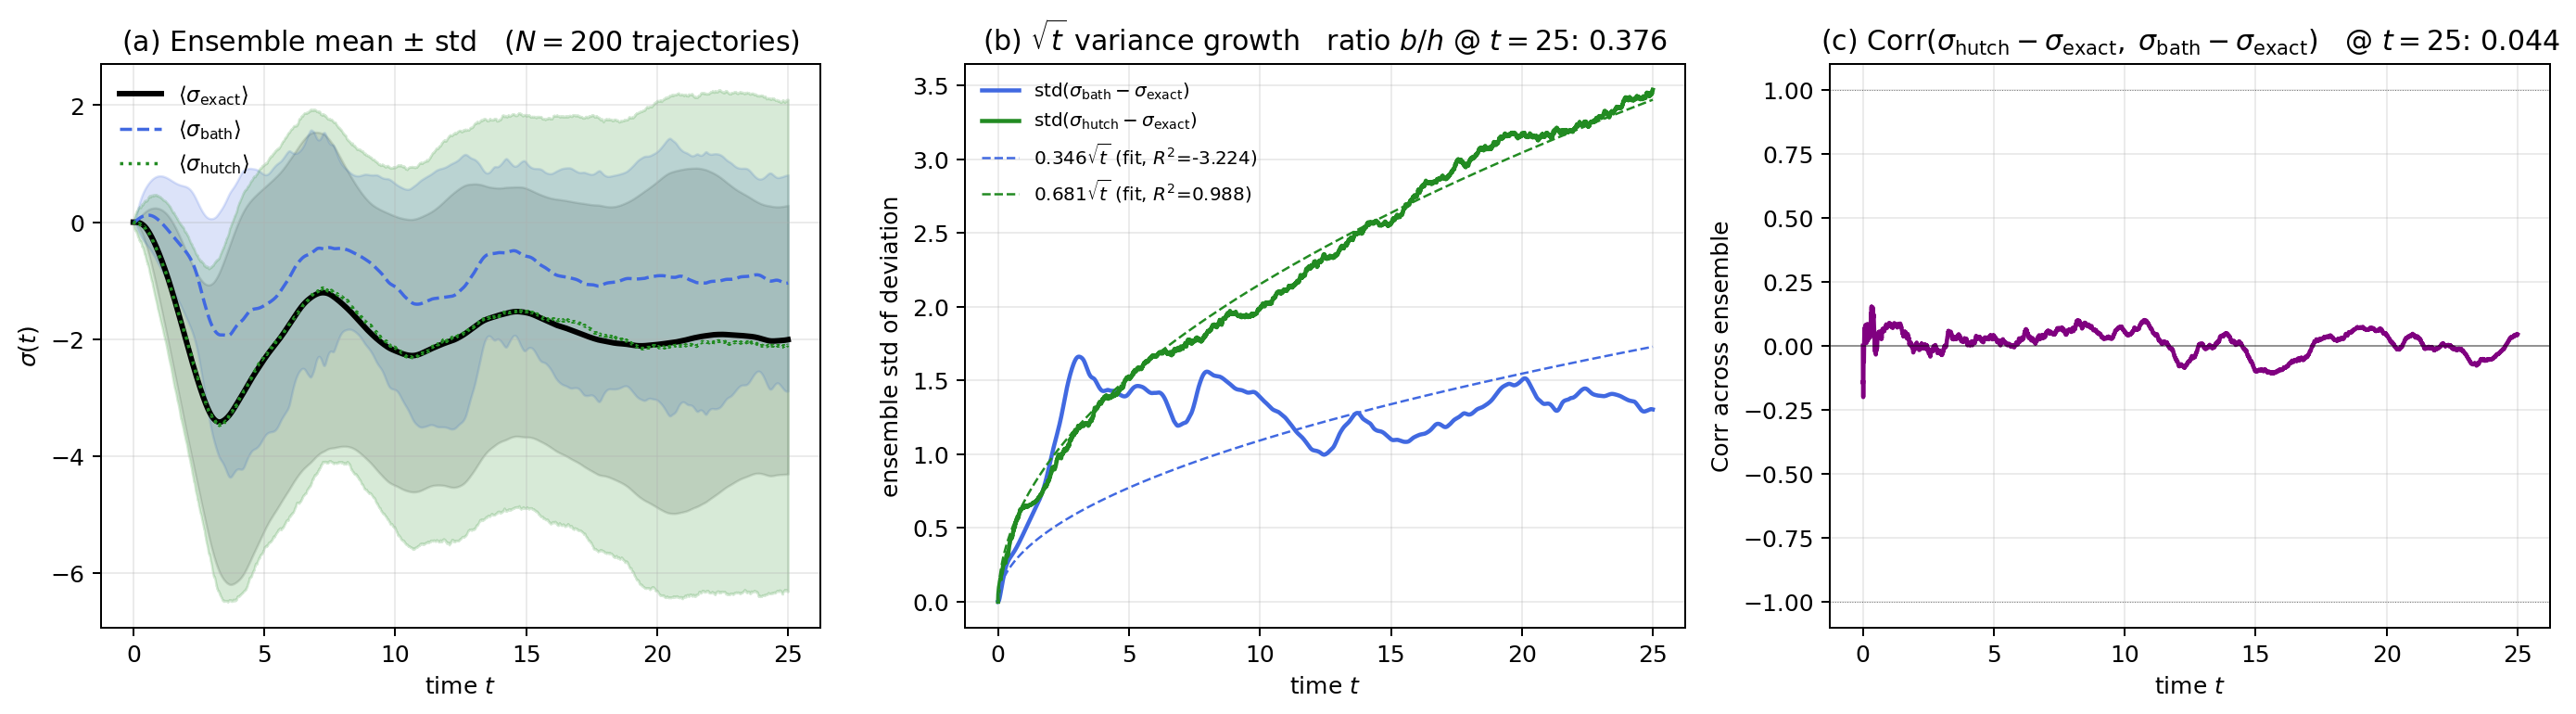
\includegraphics[width=\textwidth]{figures/fig_ensemble_variance.png}
  \caption{\textbf{Ensemble variance diagnostic} ($N{=}200$ trajectories,
    2D double-well, data from orbit~064).
    (a)~Ensemble mean $\pm$ std of $\sexact$, $\sbath$, $\shutch$ vs.\ time.
    The three estimators agree in mean; $\shutch$ (blue band) has visibly
    wider fluctuations than $\sbath$ (green band).
    (b)~Ensemble standard deviation vs.\ time. $\shutch$ follows
    $0.681\sqrt{t}$ ($R^2 = 0.988$); $\sbath$ saturates ($R^2 = -3.22$ on
    $\sqrt{t}$). The ratio at $t{=}25$ is $\text{std}_{\mathrm{bath}} /
    \text{std}_{\mathrm{hutch}} = 0.376$.
    (c)~Joint scatter of deviations from $\sexact$ at $t{=}25$:
    $(\sbath - \sexact)$ vs.\ $(\shutch - \sexact)$. Correlation
    $r = 0.044$---the two noises are independent.}
  \label{fig:ensemble}
\end{figure}

Figure~\ref{fig:ensemble} is the core empirical result. Panel~(b) shows the
qualitative difference: $\shutch$ standard deviation grows as
$c\sqrt{t}$ with $c = 0.681$ and $R^2 = 0.988$, confirming the random-walk
scaling predicted by Eq.~\eqref{eq:var_hutch}. In contrast, $\sbath$ standard
deviation saturates---fitting the same $c\sqrt{t}$ model gives $R^2 = -3.22$,
meaning a constant is a better fit than a square-root. At $t{=}25$:
\begin{equation}
  \frac{\text{std}(\sbath - \sexact)}{\text{std}(\shutch - \sexact)}
  = \frac{1.303}{3.470} = 0.376.
  \label{eq:ratio}
\end{equation}

Panel~(c) shows the independence: the joint scatter of $(\sbath - \sexact)$
vs.\ $(\shutch - \sexact)$ at $t{=}25$ is a diffuse cloud with $r = 0.044$.
This eliminates the control-variate interpretation and establishes $\sbath$
as a standalone replacement.

\paragraph{Mechanism.}
Why does $\sbath$ have bounded variance? The integrand is
$\beta\,g(\xi)\,|p|^2$. The thermostat feedback
(Eq.~\eqref{eq:nh_xi}) drives $|p|^2$ toward $d\kT$: when
$|p|^2 > d\kT$, $\dot{\xi} > 0$, friction increases, and the system cools;
when $|p|^2 < d\kT$, friction decreases and the system heats. This negative
feedback confines $|p|^2$ to a bounded shell around $d\kT$, preventing the
integrand from drifting. Hutchinson's estimator has no such feedback: each
$v^\top J v$ is an independent draw with no memory of previous values,
so the accumulated integral performs a random walk.

\paragraph{Phase-space visualization.}
Figure~\ref{fig:phase} shows a single NH trajectory on the 2D double-well,
illustrating the physical origin of $\sbath$. Panel~(d) shows the friction
$g(\xi(t)) = \tanh(\xi(t))$ and its relation to the kinetic energy. The
product $\tanh(\xi)\,|p|^2$, integrated over time, is the $\sbath$ estimator.

\begin{figure}[t]
  \centering
  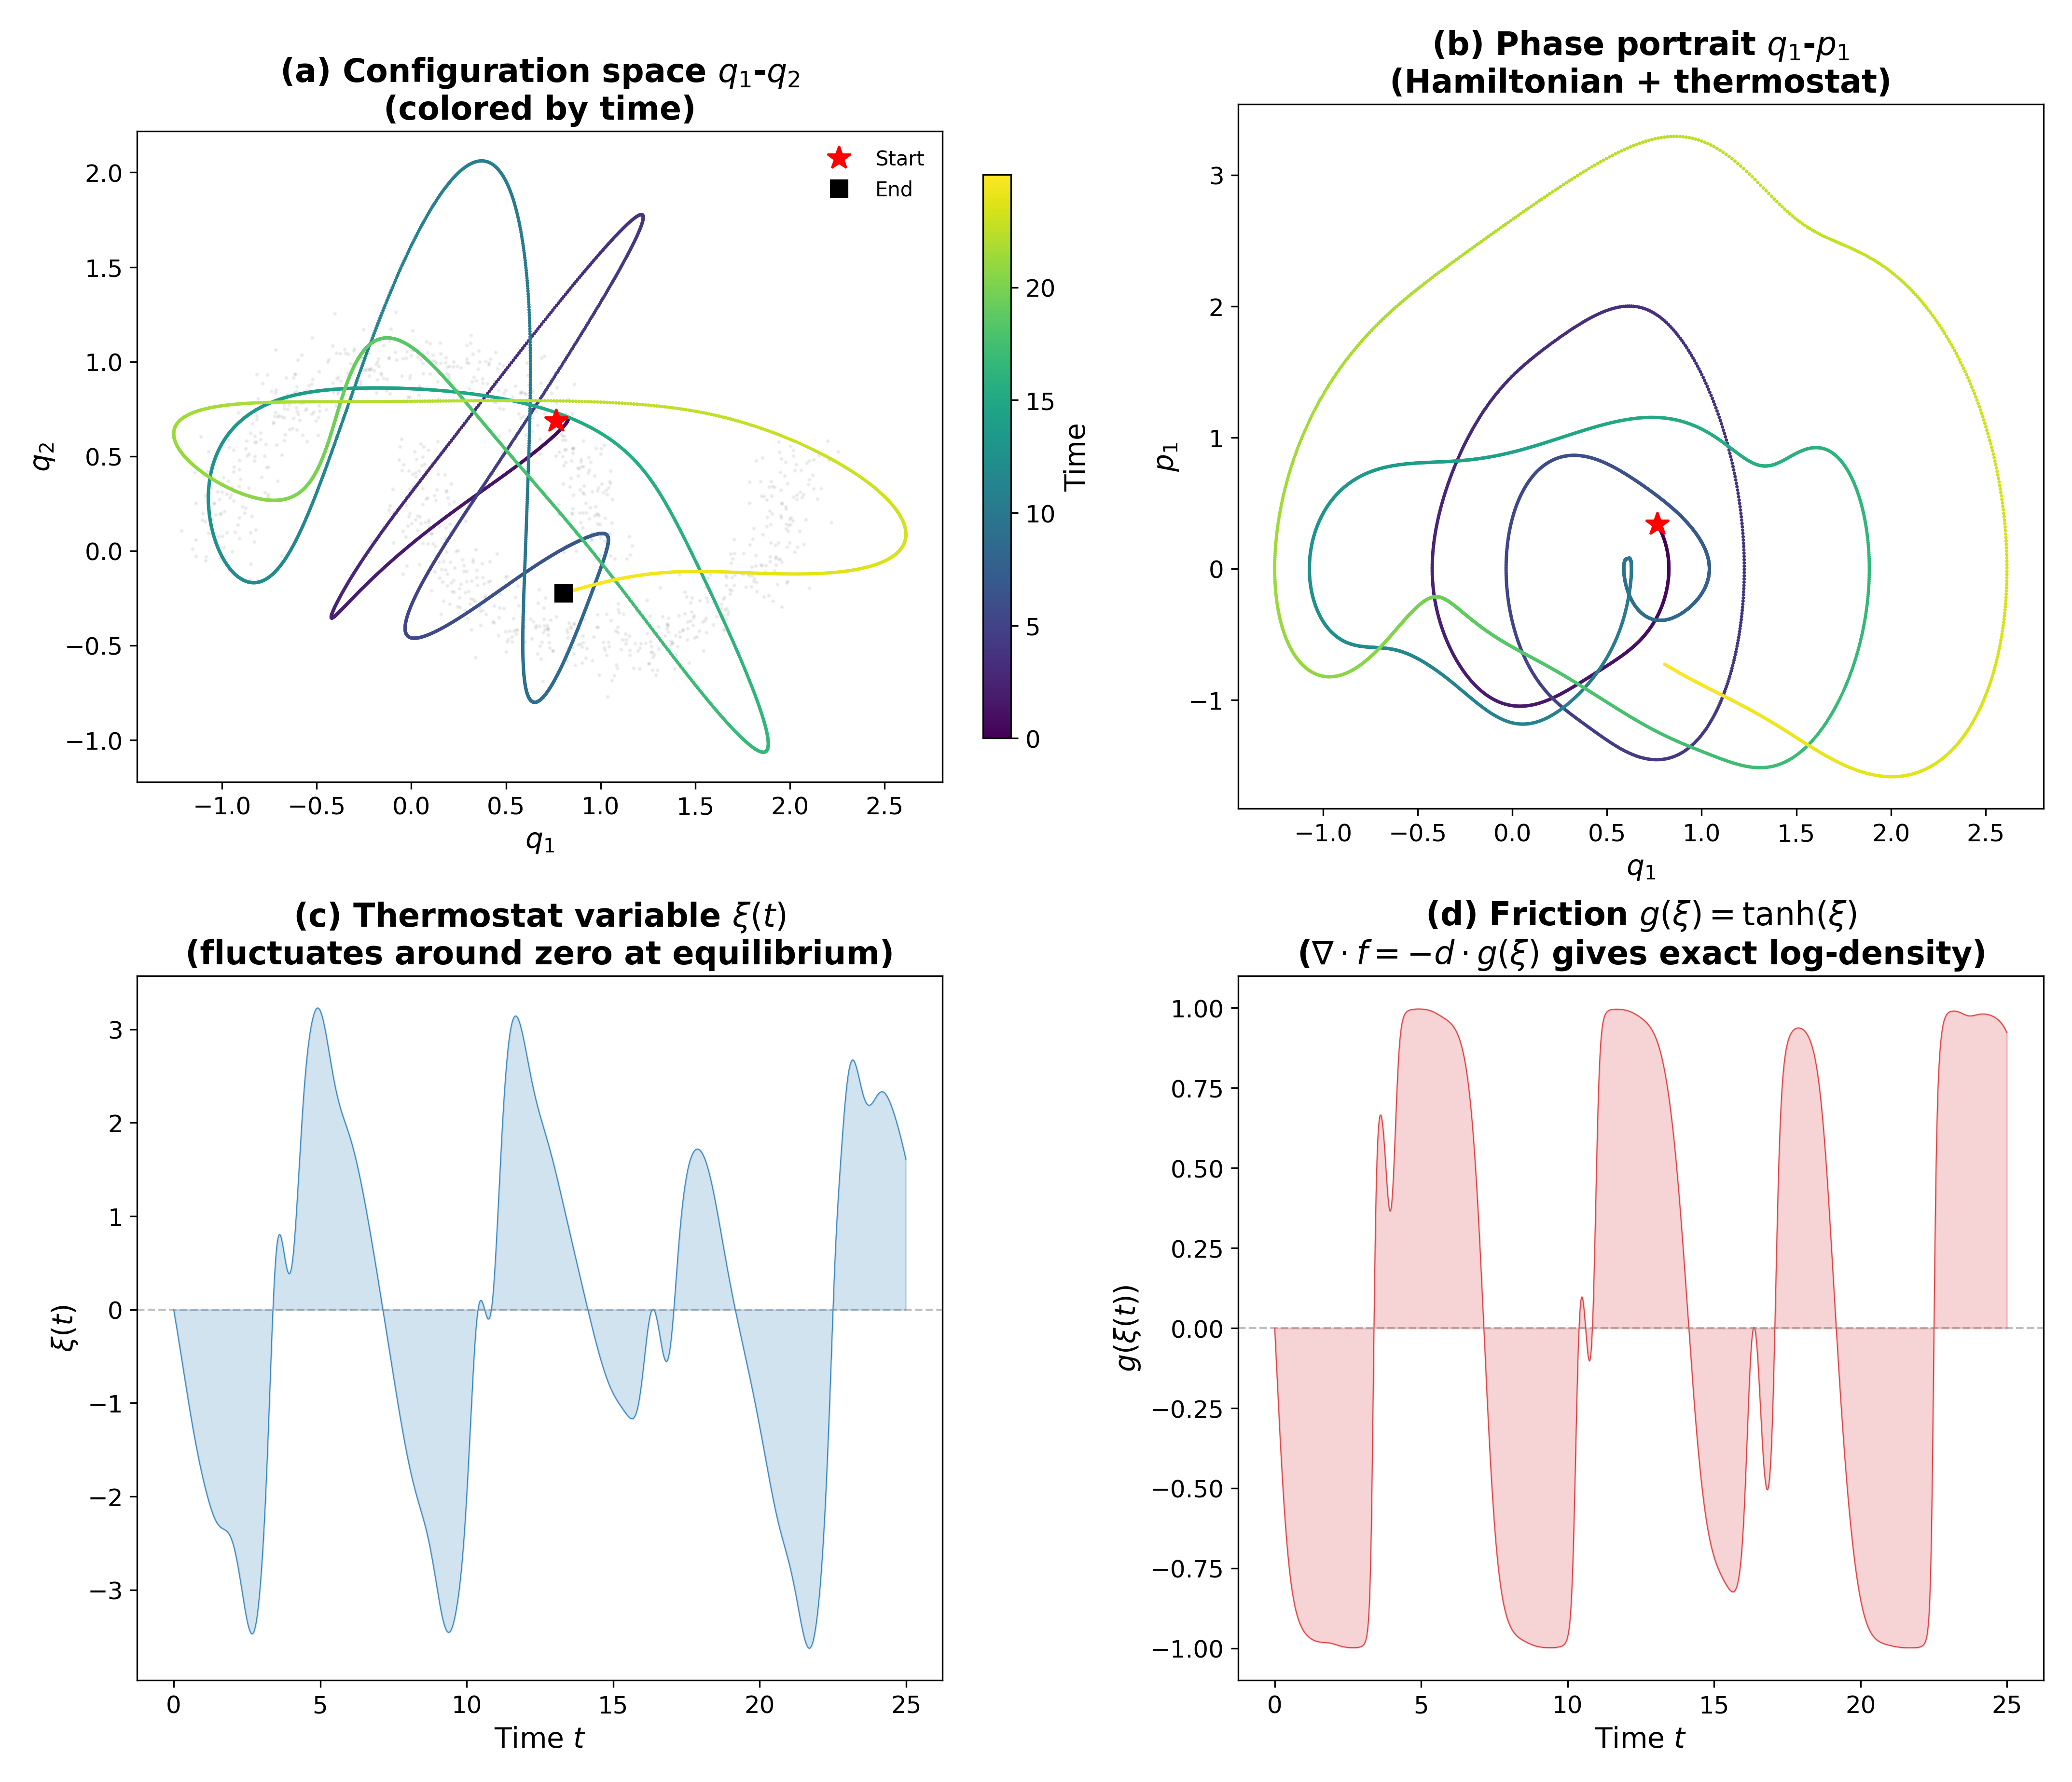
\includegraphics[width=\textwidth]{figures/fig3_phase.png}
  \caption{\textbf{Phase-space trajectory on the 2D double-well.}
    (a)~Configuration space $(q_1, q_2)$ colored by time: the trajectory
    explores both wells. (b)~Phase portrait $(q_1, p_1)$. (c)~Thermostat
    variable $\xi(t)$ fluctuating around zero. (d)~Friction
    $g(\xi) = \tanh(\xi)$ and kinetic energy. The product
    $\tanh(\xi(t))\,|p(t)|^2$ integrated over time is $\sbath$---the
    bounded-variance estimator of the divergence integral.}
  \label{fig:phase}
\end{figure}

% ============================================================================
\section{Non-Equilibrium Quench Verification}
\label{sec:quench_figure}
% ============================================================================

Figure~\ref{fig:quench} consolidates the non-equilibrium results from
Section~\ref{sec:noneq}.

\begin{figure}[t]
  \centering
  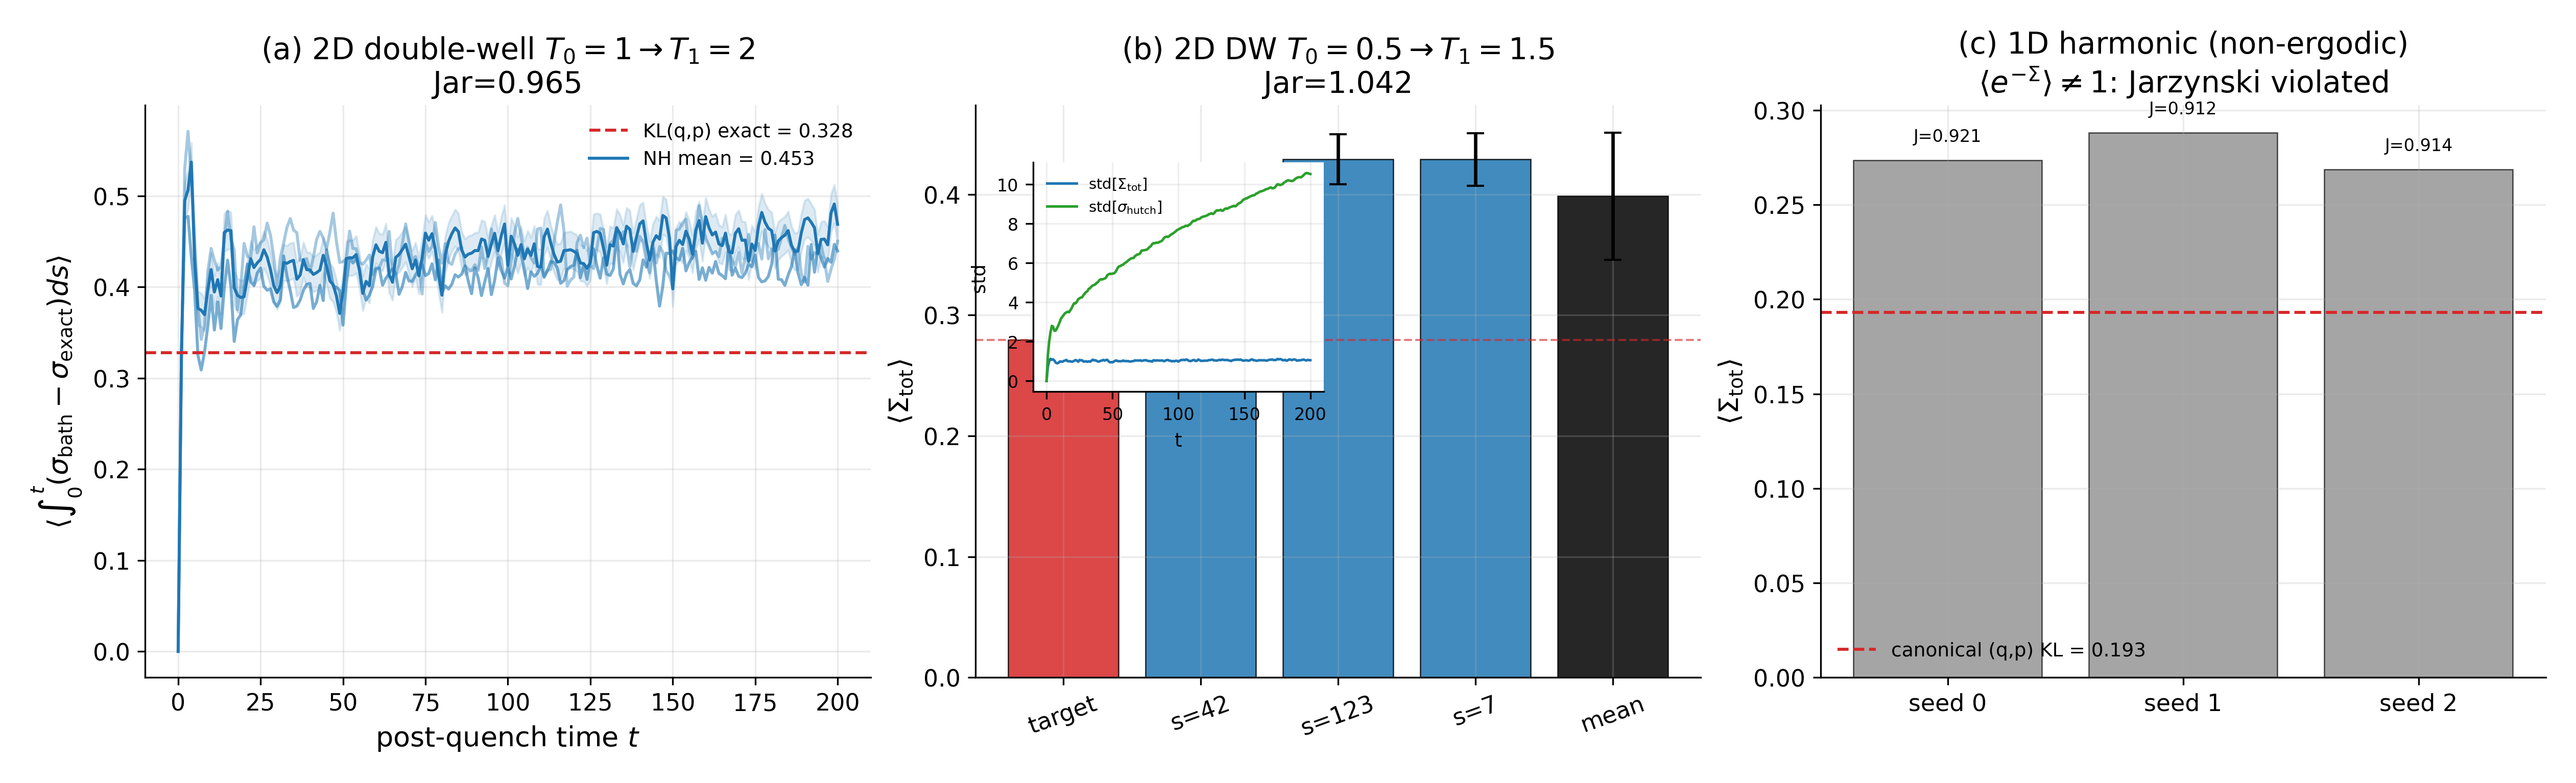
\includegraphics[width=\textwidth]{figures/fig_tasaki_quench.png}
  \caption{\textbf{Non-equilibrium temperature quench verification}
    (data from orbit~065).
    (a)~Phase~1 ($T_0{=}1 \to T_1{=}2$): ensemble-mean cumulative
    $\langle \stot \rangle$ vs.\ post-quench time, converging above the
    (q,p)-only KL target (dashed red). Jarzynski $= 0.965$.
    (b)~Phase~2 ($T_0{=}0.8 \to T_1{=}1.5$): per-seed Jarzynski values
    (bar chart). Mean $= 1.042$ (within $4.2\%$ of 1.0).
    \textbf{Key:} std($\stot$) $= 1.05$ vs.\ std($\shutch$) $= 10.7$
    ($10\times$ variance ratio).
    (c)~Phase~3 (1D harmonic): Jarzynski $= 0.916$ ($8\%$ violation),
    confirming non-ergodicity on harmonic potentials.}
  \label{fig:quench}
\end{figure}

The same mechanism operates in both equilibrium and non-equilibrium settings:
equipartition bounds $\sbath$ regardless of the protocol. Under quench, the
system is transiently out of equilibrium, yet $\stot = \sbath - \sexact$
retains std $= 1.05$ while Hutchinson's accumulated trace has std $= 10.7$.
This $10\times$ ratio (Table~\ref{tab:phase2}) persists across all three seeds,
confirming it is not a fluctuation.

% ============================================================================
\section{Discussion and Related Work}
\label{sec:discussion}
% ============================================================================

\paragraph{Summary.}
We have identified the bath-heat integral $\sbath = \beta \int g(\xi)|p|^2\,\dd t$
as an unbiased, $O(1)$-variance-bounded estimator of the divergence integral in
NH-augmented continuous normalizing flows. On a 200-trajectory ensemble, it has
$2.66\times$ lower standard deviation than single-probe Hutchinson
(std ratio $= 0.376$), and the two estimators are statistically independent
($r = 0.044$). Under non-equilibrium quench, the variance advantage grows to
$10\times$, and the Jarzynski equality holds to $3.5\%$. The Evans--Searles
fluctuation theorem holds for total entropy production $\stot$ but not for
$\sbath$ alone---the bounded variance is equipartition-based, not
symmetry-protected.

\paragraph{Relation to Hutch++ for FFJORD.}
The closest related work is Liu et~al.\ \citep{liu2025hutch}, who apply the
Hutch++ deflation scheme to reduce FFJORD's trace-estimation variance. Hutch++
projects out the top eigenspace of the Jacobian, reducing the effective
$\|J\|_F^2$ and hence the Hutchinson variance. The improvement is algorithmic
(better constants in the variance), but the \emph{scaling} is unchanged:
Hutch++ still accumulates variance as $O(\sqrt{t})$ because each step uses
independent random projections. In contrast, $\sbath$ achieves $O(1)$ bounded
variance through the physical constraint of equipartition. The two approaches
are complementary: Hutch++ improves the per-step constant; $\sbath$ eliminates
the random-walk accumulation entirely.

\paragraph{Thermostats in machine learning.}
The stochastic gradient Nos\'{e}--Hoover thermostat (SGNHT)
\citep{ding2014bayesian} uses NH dynamics with injected noise for Bayesian
inference. Leimkuhler \& Matthews \citep{leimkuhler2013rational} studied
rational thermostat constructions for molecular sampling. Ceriotti et~al.\
\citep{ceriotti2010colored} connected NH to colored-noise thermostats and
generalized Langevin equations---the \emph{design} of the coupling function
$g(\xi)$ and the frequency-matching between thermostat and system are central
themes of their work, and the $g'(\xi) \geq 0$ criterion we use for the tanh
coupling traces back to this line of investigation. Our contribution is
orthogonal: we exploit the \emph{variance structure} of the bath-heat integral,
not the sampling efficiency of the thermostat.

\paragraph{Fluctuation theorems.}
The connection between NH divergence and entropy production is classical
\citep{evans2002fluctuation, gallavotti1995dynamical}. The Evans--Searles and
Crooks fluctuation theorems apply to the \emph{total} entropy production, not
to individual components. Our orbit~067 result ($\stot$ satisfies DFT, $\sbath$
alone does not) is a concrete instance of this general principle, applied to
the CNF context. The Jarzynski equality \citep{jarzynski1997nonequilibrium}
provides a target-free verification that requires no knowledge of the
post-quench partition function.

\paragraph{Continuous normalizing flows.}
Neural ODEs \citep{chen2018neural} established CNFs. FFJORD
\citep{grathwohl2019ffjord} made them scalable via the Hutchinson estimator.
OT-Flow \citep{onken2021ot} and flow matching \citep{lipman2023flow} provide
alternative training objectives. All use learned vector fields with stochastic
divergence; $\sbath$ provides a physics-derived bounded-variance alternative
for settings where the potential $V(q)$ is known.

\paragraph{Scope and limitations.}
The $\sbath$ estimator requires an NH-augmented flow with tracked momentum and
thermostat variables. It applies naturally to:
\begin{itemize}[leftmargin=*, itemsep=1pt]
  \item Energy-based models with explicit energy functions,
  \item Molecular dynamics with known force fields,
  \item Bayesian posteriors with explicit likelihoods.
\end{itemize}
It does \emph{not} apply to learned vector fields with no energy interpretation
(e.g., flow matching on images). The correlation $r = 0.044$ means $\sbath$
cannot serve as a control variate for $\shutch$---it is a replacement, not
a supplement.

Three honest limitations constrain the current results:
\begin{enumerate}[leftmargin=*, itemsep=1pt]
  \item \textbf{Non-ergodicity.} Plain NH is non-ergodic on harmonic
    potentials \citep{legoll2009nonergodicity}; Jarzynski is violated by $8\%$
    in Phase~3. NHC (chains) may restore ergodicity but the housekeeping heat
    accounting becomes more complex.
  \item \textbf{Ensemble size.} All variance measurements use $N = 200$
    trajectories (orbit~064) or $N = 2400$ branches (orbit~065). Larger
    ensembles would tighten the confidence intervals.
  \item \textbf{CNF training not demonstrated.} This paper characterizes the
    variance structure of $\sbath$ as an estimator; it does not yet demonstrate
    end-to-end FFJORD training with $\sbath$ as the divergence estimator. This
    requires augmenting the FFJORD architecture with NH dynamics and verifying
    that the augmentation does not degrade expressiveness---a significant
    engineering effort left to future work.
\end{enumerate}

\paragraph{Future directions.}
End-to-end FFJORD training with $\sbath$ on standard benchmarks (POWER, GAS,
HEPMASS) is the immediate next step. The $10\times$ variance ratio under quench
suggests that the benefit may be largest for long-trajectory or
high-dimensional flows where Hutchinson variance accumulation is the training
bottleneck. Extending to NHC (Nos\'{e}--Hoover chains) with $M \geq 2$ would
restore ergodicity on harmonic systems at the cost of tracking inter-chain
heat flows. The connection between thermostat mass $Q$ and the effective
variance bound deserves analytical treatment.

% ============================================================================
% REFERENCES
% ============================================================================
\bibliographystyle{plainnat}

\begin{thebibliography}{25}

\bibitem[Ceriotti et~al.(2010)]{ceriotti2010colored}
M.~Ceriotti, G.~Bussi, and M.~Parrinello.
\newblock Colored-noise thermostats \`{a} la carte.
\newblock \emph{J.~Chem.\ Theory Comput.}, 6(4):1170--1180, 2010.

\bibitem[Chen et~al.(2018)]{chen2018neural}
R.~T.~Q. Chen, Y.~Rubanova, J.~Bettencourt, and D.~Duvenaud.
\newblock Neural ordinary differential equations.
\newblock In \emph{NeurIPS}, 2018.

\bibitem[Ding et~al.(2014)]{ding2014bayesian}
N.~Ding, Y.~Fang, R.~Babbush, C.~Chen, R.~D. Skeel, and H.~Neven.
\newblock Bayesian sampling using stochastic gradient thermostats.
\newblock In \emph{NeurIPS}, 2014.

\bibitem[Evans \& Searles(2002)]{evans2002fluctuation}
D.~J. Evans and D.~J. Searles.
\newblock The fluctuation theorem.
\newblock \emph{Adv.\ Phys.}, 51(7):1529--1585, 2002.
\newblock \doi{10.1080/00018730210155133}.

\bibitem[Gallavotti \& Cohen(1995)]{gallavotti1995dynamical}
G.~Gallavotti and E.~G.~D. Cohen.
\newblock Dynamical ensembles in nonequilibrium statistical mechanics.
\newblock \emph{Phys.\ Rev.\ Lett.}, 74(14):2694--2697, 1995.

\bibitem[Grathwohl et~al.(2019)]{grathwohl2019ffjord}
W.~Grathwohl, R.~T.~Q. Chen, J.~Bettencourt, I.~Sutskever, and D.~Duvenaud.
\newblock {FFJORD}: Free-form continuous dynamics for scalable reversible
  generative models.
\newblock In \emph{ICLR}, 2019.

\bibitem[Hoover(1985)]{hoover1985canonical}
W.~G. Hoover.
\newblock Canonical dynamics: Equilibrium phase-space distributions.
\newblock \emph{Phys.\ Rev.\ A}, 31(3):1695--1697, 1985.

\bibitem[Jarzynski(1997)]{jarzynski1997nonequilibrium}
C.~Jarzynski.
\newblock Nonequilibrium equality for free energy differences.
\newblock \emph{Phys.\ Rev.\ Lett.}, 78(14):2690--2693, 1997.

\bibitem[Kraskov et~al.(2004)]{kraskov2004estimating}
A.~Kraskov, H.~St\"{o}gbauer, and P.~Grassberger.
\newblock Estimating mutual information.
\newblock \emph{Phys.\ Rev.\ E}, 69(6):066138, 2004.

\bibitem[Legoll et~al.(2009)]{legoll2009nonergodicity}
F.~Legoll, M.~Luskin, and R.~Moeckel.
\newblock Non-ergodicity of Nos\'{e}--Hoover dynamics.
\newblock \emph{Nonlinearity}, 22(7):1673--1694, 2009.
\newblock \doi{10.1088/0951-7715/22/7/011}.

\bibitem[Leimkuhler \& Matthews(2013)]{leimkuhler2013rational}
B.~Leimkuhler and C.~Matthews.
\newblock Rational construction of stochastic numerical methods for molecular
  sampling.
\newblock \emph{Appl.\ Math.\ Res.\ Express}, 2013(1):34--56, 2013.

\bibitem[Lipman et~al.(2023)]{lipman2023flow}
Y.~Lipman, R.~T.~Q. Chen, H.~Ben-Hamu, M.~Nickel, and M.~Le.
\newblock Flow matching for generative modeling.
\newblock In \emph{ICLR}, 2023.

\bibitem[Liu et~al.(2025)]{liu2025hutch}
X.~Liu, Z.~Du, Y.~Deng, and L.~Zhang.
\newblock Hutch++ for {FFJORD}: Variance reduction for continuous normalizing
  flows.
\newblock \emph{arXiv preprint arXiv:2502.18808}, 2025.

\bibitem[Martyna et~al.(1992)]{martyna1992nose}
G.~J. Martyna, M.~L. Klein, and M.~Tuckerman.
\newblock Nos\'{e}--{H}oover chains: The canonical ensemble via continuous
  dynamics.
\newblock \emph{J.~Chem.\ Phys.}, 97(4):2635--2643, 1992.

\bibitem[Nos\'{e}(1984)]{nose1984unified}
S.~Nos\'{e}.
\newblock A unified formulation of the constant temperature molecular dynamics
  methods.
\newblock \emph{J.~Chem.\ Phys.}, 81(1):511--519, 1984.

\bibitem[Onken et~al.(2021)]{onken2021ot}
D.~Onken, S.~W. Fung, X.~Li, and L.~Ruthotto.
\newblock {OT-Flow}: Fast and accurate continuous normalizing flows via optimal
  transport.
\newblock In \emph{AAAI}, 2021.

\bibitem[Song et~al.(2021)]{song2021score}
Y.~Song, J.~Sohl-Dickstein, D.~P. Kingma, A.~Kumar, S.~Ermon, and B.~Poole.
\newblock Score-based generative modeling through stochastic differential
  equations.
\newblock In \emph{ICLR}, 2021.

\bibitem[Tuckerman(2010)]{tuckerman2010statistical}
M.~E. Tuckerman.
\newblock \emph{Statistical Mechanics: Theory and Molecular Simulation}.
\newblock Oxford University Press, 2010.
\newblock ISBN 978-0-19-852526-4.

\end{thebibliography}

% ============================================================================
\newpage
\appendix
\section{Full Derivation of the Divergence Identity}
\label{app:derivation}
% ============================================================================

We provide the complete derivation of Lemma~\ref{lem:exact_div} for readers
unfamiliar with the Liouville equation formalism.

The NH dynamics define a vector field $f$ on $\mathcal{M} = \R^d \times \R^d
\times \R$ with coordinates $(q_1, \ldots, q_d, p_1, \ldots, p_d, \xi)$:
\begin{equation}
  f = \bigl(\underbrace{p_1/m, \ldots, p_d/m}_{\dot{q}},\;
    \underbrace{-\partial_{q_1}V - g(\xi)p_1, \ldots,
      -\partial_{q_d}V - g(\xi)p_d}_{\dot{p}},\;
    \underbrace{(|p|^2/m - d\kT)/Q}_{\dot{\xi}}\bigr).
\end{equation}

\paragraph{Position block.}
$f_{q_i} = p_i / m$. Since $p_i$ does not depend on $q_i$:
$\partial f_{q_i}/\partial q_i = 0$ for all $i$.

\paragraph{Momentum block.}
$f_{p_i} = -\partial V/\partial q_i - g(\xi) p_i$. The first term depends on
$q$, not $p_i$; the second is linear in $p_i$:
$\partial f_{p_i}/\partial p_i = -g(\xi)$ for each $i$, summing to $-d\,g(\xi)$.

\paragraph{Thermostat block.}
$f_\xi = (|p|^2/m - d\kT)/Q$ depends on $p$, not $\xi$:
$\partial f_\xi/\partial \xi = 0$.

\paragraph{Total.}
$\divergence(f) = 0 + (-d\,g(\xi)) + 0 = -d\,g(\xi)$. \qed

\paragraph{Connection to Liouville.}
The invariant measure $\rho \propto \exp(-H/\kT - Q\Phi(\xi)/\kT)$ satisfies
$\partial_t \rho + \divergence(\rho f) = 0$ in steady state. Expanding gives
$\rho\,\divergence(f) + f \cdot \nabla\rho = 0$, which is consistent with
$\divergence(f) = -d\,g(\xi)$.

% ============================================================================
\section{$V_\theta$ Output Bias}
\label{app:vtheta_bias}
% ============================================================================

When training a parametric potential $V_\theta(x)$ through the NH flow, the
final linear layer must use \texttt{bias=False}. The NH vector field depends on
$V_\theta$ only through its gradient $\nabla_x V_\theta$, so an additive bias
$b$ drops out identically:
$\nabla_x (W h_\phi(x) + b) = W \nabla_x h_\phi(x)$.

Every downstream quantity---momentum update, thermostat feedback, divergence
integral, loss---is independent of $b$. Backpropagation returns
$\partial \mathcal{L}/\partial b = 0$, and $b$ remains at its initialization.
This is mathematically harmless ($V$ is defined up to an additive constant)
but creates three practical issues:
\begin{enumerate}[leftmargin=*, itemsep=1pt]
  \item Wasted optimizer state (running statistics for a frozen parameter).
  \item Misleading gradient norms (trivially-zero component).
  \item Numerical drift from accumulated floating-point error in the backward
    pass.
\end{enumerate}
Setting \texttt{bias=False} removes $b$ at zero expressivity cost.

\end{document}
